\chapter{Problema}

\section{Definirea problemei}

\paragraph{}
Problema pe care am încercat să o rezolv constă în primul rând în a urmări cu acuratețe ochii utilizatorului, astfel încât cursorul să poată fi mișcat în concordanță cu privirea acestuia.
Această problemă face parte dintr-o gamă mai largă de probleme de \emph{Viziune Computerizată} (în engleză \emph{Computer Vision}), mai exact \emph{Urmărirea ochilor}, după cum a fost menționat și în introducere.
Conform \cite{eye_tracking}, urmărirea ochilor este ``procesul de măsurare a punctului de privire (unde se uită o persoană) sau a mișcării unui ochi relativ la cap''.\footnote{Textul original este din engleză: ``the process of measuring either the point of gaze (where one is looking) or the motion of an eye relative to the head''}

\paragraph{}
Tehnicile de ultimă oră (\emph{state of the art}) de a rezolva această problemă se bazează pe \emph{Inteligența Artificială} și sunt, mai exact, tehnici de \emph{Învățare Automată}.
\cite{liviu_ciortuz_ml} explică în termeni foarte simpli acest subdomeniu al informaticii: ``Învățarea Automată este programare bazată pe date''\footnote{Traducere liberă; text original: ``ML is data-driven programming''}.
Învățarea poate fi la rândul ei supervizată, semi-supervizată sau nesupervizată, aceste tehnici încearcând să prezică, să producă, să generalizeze niște rezultate pe baza unor exemple sau a unor relații dintr-o mulțime de date deja cunoscută.
Diferența cheie între acestea constă în structura acestei mulțimi de date, structură care la rândul ei influențează abordările de învățare.

\paragraph{}
În acest caz, m-am concentrat asupra învățării supervizate, care presupune cunoașterea unei mulțimi de date $$D = \{(i, o) | i \in I, o \in O\}$$
unde $i$ reprezintă o instanță, un exemplu care conține o informație care trebuie prezisă, calculată, iar $o$ reprezintă acea informație, un \emph{adevăr de bază} deja cunoscut.
Astfel, primul pas spre rezolvarea problemei este \emph{colectarea datelor de antrenament}.

\paragraph{}
TODO <--------------------- asta de mutat in cap 2, la adunare de date
Pentru această aplicație, mulțimea $I$ de mai sus va fi alcătuită din imagini alea utilizatorului, iar mulțimea $O$ va conține, spre exemplu, coordonatele $(x, y)$ ale poziției la care se uita utilizatorul pe ecran atunci când acea imagine va fi capturată.
Vom considera că pentru orice imagine din mulțimea $I$ nu conține imagini în care utilizatorul nu se uita la ecran.

\paragraph{}
Învățarea profundă se preocupă, printre altele, de procesarea și analizarea imaginilor prin folosirea unor \emph{arhitecturi profunde} bazate pe \emph{rețele neuronale}.
Învățarea poate fi la rândul ei supervizată, semi-supervizată sau nesupervizată.
În termeni simpli, aceste tehnici încearcă să prezică sau să producă un rezultat pe baza unor exemple sau a unor relații între datele care trebuiesc procesate.

\subsection{Neuronul Artificial}
\paragraph{}
Înainte de a analiza arhitecturi de învățare profundă mai sofisticate, trebuie să aruncăm o privire rapidă asupra neuronului artificial.
Pe scurt, este un model formal, simplificat al unui neuron biologic.
Ne poate ajuta să realizăm \emph{clasificare binară} folosind următoarea formulă:
$$
y = \varphi (w * x + b)
$$
% \begin{equation}
%     f(x) =
%     \begin{cases}
%       1, & \text{if}\ w * x + b > 0 \\
%       0, & \text{autrement}
%     \end{cases}
% \end{equation}

\paragraph{}
În formula de mai sus, $x$ este un vector de valori reale, reprezentând datele de intrare, iar $w$ este un vector de valori reale denumit \emph{vectorul ponderilor} (în engleză \emph{weights}) și $b$ este \emph{parțialitatea} (în engleză \emph{bias-ul}).
Produsul $w * x$ reprezintă produsul scalar și este egal cu $w * x = \sum _{i=1}^{n}w_{i}x_{i}$, $n$ fiind lungimea vectorului $x$.

\paragraph{}
Rezultatul clasificării este dat de $\varphi$, denumit \emph{funcție de activare}.
Daca aceasta se comportă ca un prag, o limită, un \emph{threshold}, atunci funcția de activare se va traduce într-o clasificare binară, cu rezultat $0$ sau $1$.
Putem folosi și $\varphi(x) = x$, ecuație care ne poate ajuta la rezolvarea problemelor de tip \emph{regresie liniară}.

\begin{figure}[h]
    \centering
    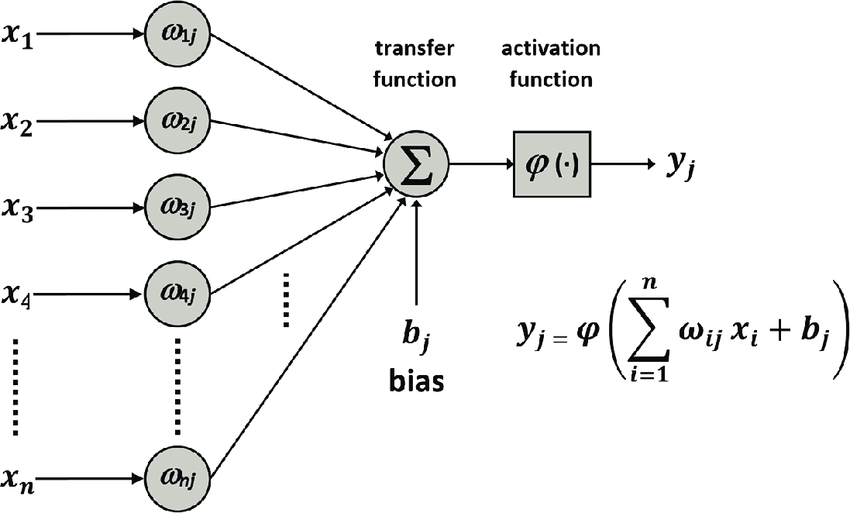
\includegraphics[width=\textwidth]{artificial_neuron.png}
    \caption{Algoritmul perceptron, bazat pe neuronul artificial. Imagine preluată de pe site-ul \href{https://www.researchgate.net/figure/Scheme-of-a-perceptron-A-nonlinear-activation-function-BULLET-is-applied-to-the_fig3_315788933}{ResearchGate}}
\end{figure}


\subsection{Rețele neuronale}
\paragraph{}
``Calul de bătaie'' pentru problemele de Viziune Computerizată este Rețeaua Neuronală Artificială.
Ea este, dupa cum sugerează și numele, compusă din mai multi neuroni artificiali, distribuiți pe mai multe \emph{straturi}.

\begin{figure}[h]
    \centering
    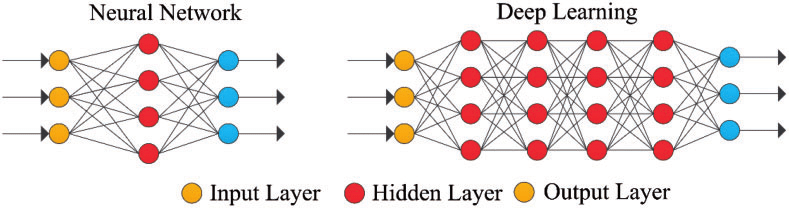
\includegraphics[width=\textwidth]{ann.png}
    \caption{Structură generală a unei rețele neuronale. Imagine preluată de pe site-ul \href{https://www.researchgate.net/figure/Deep-learning-diagram_fig5_323784695}{ResearchGate}}
\end{figure}

\section{Strategie}

\subsection{Obținerea datelor de antrenament}
\paragraph{}
Este foarte bine cunoscut că un algoritm de Învățare Automată este pe atât de bun pe cât sunt datele pe care i le furnizăm.
Acestea sunt incredibil de importante, așa că m-am concentrat pe a dezvolta niște modalități facile de a aduna o mulțime consistentă de date

\paragraph{}
O altă etapă esențială este \emph{procesarea de date}.
Aceasta se preocupă cu simplificarea și curățarea setului de date, cu eliminarea instanțelor de antrenament care sunt inutile și cu extragerea exclusiv a informațiilor care sunt de folos și cu înlăturarea a ceea ce rămâne.
Opțional, în această etapă se mai realizează și diferite transformări pentru a aduce datele dintr-o formă neprelucrată într-o formă convenabilă algoritmilor pe care îi folosim.

\subsection{Rețeaua de tip perceptron multistrat}
\paragraph{}
Un tip special de rețea neuronală este \emph{Perceptronul Multistrat} (\emph{Multilayer Perceptron Network}).
Am folosit această arhitectură ca un punct de pornire spre a rezolva problema și ca un prim experiment.

\paragraph{}
Folosind acest tip de rețea, am încercat să ating cel mai important obiectiv al acestei lucrări al licenței, și anume de a prezice aproximativ zona în care se uită utilizatorul, pentru a putea deplasa cursorul în acea zonă.
Din experimentele efectuate, această arhitectură a rezultat într-o primă soluție promițătoare, fiind capabilă să urmărească, într-o anumită măsura, privirea utilizatorului.

\subsection{Rețele neuronale convoluționale}
\paragraph{}
Un următor pas a fost studierea și aplicarea \emph{rețelelor neuronale convoluționale}, o arhitectură de bază pentru multe metode ``state of the art'' pentru problemele din domeniul Viziunii Computerizate.
Cu ajutorul acestora, urmărirea ochilor a devenit mai robustă și mai puțin sensibilă la diferențele dintre imagini, precum lumină sau poziționare.

\subsection{Cercetare și analizare a bibliotecilor folosite}
\paragraph{}
În lucrarea de licență am folosit diverse biblioteci printre care și \lstinline{dlib}, pe care am folosit-o pentru a identifica reperele faciale ale utilizatorului.
Am fost curios despre cum anume funcționează această bibliotecă și am făcut un mic experiment în care am încercat să reconstruiesc funcționalitatea acestei librării.